Se puede añadir texto antes de empezar la primera sección.


\section{Contexto y alcance}

Esta memoria representa el trabajo realizado para desarrollar la aplicación web de CoWordle, que ademas representa el trabajo de fin de grado de Jorge Moreno Fernández.
El objetivo de este trabajo era conseguir realizar una aplicación web interactuable en tiempo real utilizando websockets y las últimas tecnologias web.


\section{Estructura del documento}

La estructura del TFG no es fija. El tutor indicará una estructura adecuada dependiendo del trabajo concreto.\tutor{Comentario del tutor}

Se puede incluir dentro de cada apartado secciones adicionales. La copia en papel de la memoria del TFG será encuadernada en pasta dura de color azul (p.e. encuadernación tipo chanel). La portada, que puede ser una pegatina transparente, seguirá el modelo que se adjunta, que incluye el escudo y nombre de la URJC, la titulación cursada por el alumno, el curso académico, el título del TFG, el autor y el o los directores/tutores.\alumno{Comentario del alumno}

\section{La idea}
CoWordle es un juego multijugador derivado de Wordle, que añade a la versión original la capacidad de jugar en tiempo real con otros jugadores.


\section{Wordle}
Wordle es un juego de navegador creado por el ingeniero Josh Wardle.

\subsection{La historia de Wordle}

TODO

\subsection{¿Comó se juega?}

Wordle es un juego en el que cada día, todos los jugadores del mundo tienen que descubrir la misma palabra.
Cada jugador tiene seis oportunidades para encontrar la palabra secreta, y cada oportunidad ofrece pistas sobre lo bien que has colocado cada letra del intento.

El juego utiliza colores como pistas para cada letra del intento:
\begin{itemize}
	\item El color gris indica que la letra no se encuentra en la palabra objetivo.
	\item El color naranja indica que la letra se encuentra en la palabra, pero no está en su posición correcta.
	\item El color verde indica que la letra se encuentra tanto en la palabra, como en la posición de la palabra correcta.
\end{itemize}

Cuando un jugador ha descubierto todas las letras de la palabra objetivo antes de quedarse sin intentos, el juego se termina y se muestra al jugador el resultado de la partida, mostrando entre otras estadísticas, el número de intentos requeridos.

Esta estadística ha sido uno de los grandes éxitos del juego, millones de jugadores intentan cada día conseguir la palabra en el menor número de intentos posibles, y comparan entre ellos los resultados con las integración de Facebook y Twitter de las que dispone la aplicación oficial.


\subsection{Otras aplicaciones derivados de Wordle}

Tras el éxito de Wordle, multitud de aplicaciones comenzaron a aparecer que clonaban las mismas mecánicas que Wordle, entre ellas, existen versiones en diferentes lenguajes o versiones donde tienes que resolver múltiples palabras simultáneamente (Octordle).

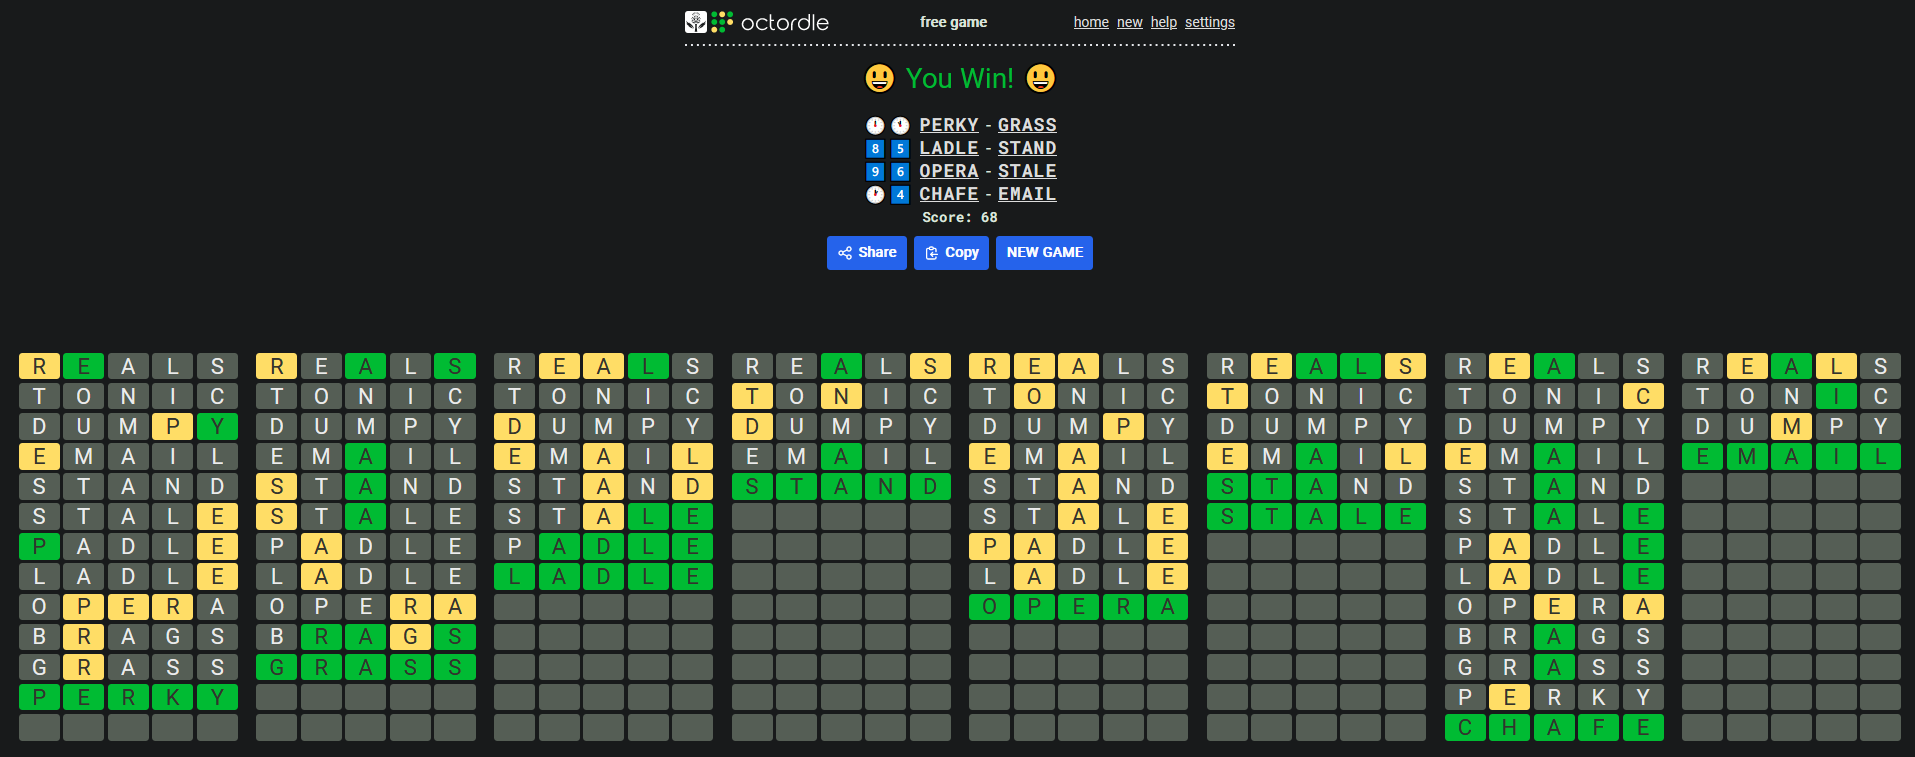
\includegraphics[clip=true,width=\textwidth]{images/octordle.png}
